\documentclass[
	12pt,
	]{article}
		\usepackage{xcolor}
			\usepackage[dvipsnames]{xcolor}
			\usepackage[many]{tcolorbox}
		\usepackage{changepage}
		\usepackage{titlesec}
		\usepackage{caption}
		\usepackage{mdframed, longtable}
		\usepackage{mathtools, amssymb, amsfonts, amsthm, bm,amsmath} 
		\usepackage{array, tabularx, booktabs}
		\usepackage{graphicx,wrapfig, float, caption}
		\usepackage{tikz,physics,cancel, siunitx, xfrac}
		\usepackage{graphics, fancyhdr}
		\usepackage{lipsum}
		\usepackage{xparse}
		\usepackage{thmtools}
		\usepackage{mathrsfs}
		\usepackage{undertilde}
		\usepackage{tikz}
		\usepackage{fullpage,enumitem,bbm}
		\usepackage[labelfont=bf]{caption}
	\newcommand{\td}{\text{dim}}
	\newcommand{\tvw}{T : V\xrightarrow{} W }
	\newcommand{\ttt}{\widetilde{T}}
	\newcommand{\ex}{\textbf{Example}}
	\newcommand{\aR}{\alpha \in \mathbb{R}}
	\newcommand{\abR}{\alpha \beta \in \mathbb{R}}
	\newcommand{\un}{u_1 , u_2 , \dots , n}
	\newcommand{\an}{\alpha_1, \alpha_2, \dots, \alpha_2 }
	\newcommand{\sS}{\text{Span}(\mathcal{S})}
	\newcommand{\sSt}{($\mathcal{S}$)}
	\newcommand{\la}{\langle}
	\newcommand{\ra}{\rangle}
	\newcommand{\Rn}{\mathbb{R}^{n}}
	\newcommand{\R}{\mathbb{R}}
	\newcommand{\Rm}{\mathbb{R}^{m}}
	\usepackage{fullpage, fancyhdr}
	\newcommand{\La}{\mathcal{L}}
	\newcommand{\ep}{\epsilon}
	\newcommand{\de}{\delta}
	\usepackage[math]{cellspace}
		\setlength{\cellspacetoplimit}{3pt}
		\setlength{\cellspacebottomlimit}{3pt}
	\newcommand\numberthis{\addtocounter{equation}{1}\tag{\theequation}}


	\usepackage{mathtools}
	\DeclarePairedDelimiter{\norm}{\lVert}{\rVert}
	\newcommand{\vectorproj}[2][]{\textit{proj}_{\vect{#1}}\vect{#2}}
	\newcommand{\vect}{\mathbf}
	\newcommand{\uuuu}{\sum_{i=1}^{n}\frac{<u,u_i}{<u_i,u_i>} u_i}
	\newcommand{\B}{\mathcal{B}}
	\newcommand{\Ss}{\mathcal{S}}
	
	\newtheorem{theorem}{Theorem}[section]
	\theoremstyle{definition}
	\newtheorem{corollary}{Corollary}[theorem]
	\theoremstyle{definition}
	\newtheorem{lemma}[theorem]{Lemma}
	\theoremstyle{definition}
	\newtheorem{definition}{Definition}[section]
	\theoremstyle{definition}
	\newtheorem{Proposition}{Proposition}[section]
	\theoremstyle{definition}
	\newtheorem*{example}{Example}
	\theoremstyle{example}
	\newtheorem*{note}{Note}
	\theoremstyle{note}
	\newtheorem*{remark}{Remark}
	\theoremstyle{remark}
	\newtheorem*{example2}{External Example}
	\theoremstyle{example}
	
	\title{PHYS 350 Assignment 2}
	\titleformat*{\section}{\LARGE\normalfont\fontsize{12}{12}\bfseries}
	\titleformat*{\subsection}{\Large\normalfont\fontsize{10}{15}\bfseries}
	\author{Mihail Anghelici 260928404 }
	\date{\today}
	
	\relpenalty=9999
			\binoppenalty=9999
		
			\renewcommand{\sectionmark}[1]{%
			\markboth{\thesection\quad #1}{}}
			
			\fancypagestyle{plain}{%
			  \fancyhf{}
			  \fancyhead[L]{\rule[0pt]{0pt}{0pt} Assignment 2 } 
			  \fancyhead[R]{\small Mihail Anghelici $260928404$} 
			  \fancyfoot[C]{-- \thepage\ --}
			  \renewcommand{\headrulewidth}{0.4pt}}
			\pagestyle{plain}
			\setlength{\headsep}{1cm}
	\captionsetup{margin =1cm}
	\begin{document}
	\maketitle
		\section*{Question 2.10}
			Since the charge is not at the center symmetry is broken. To restore symmetry we add $3$ cubes on each side of the corner charge and $4$ cubes symmetricaly on the bottom , such that now the charge is at the center. The flux flowing through the inner parts of the cubes is $0$ such that only the outward surface parts of each cube contribute to flux ($\Phi_{\text{positive,flux}} = \frac13 \Phi_{\text{one cube}}$). Moreover, because of symmetry ,each cube has an equal amount of flux ($\Phi_{one cube} = \frac18 \Phi_{E}$). It follows that 
			$$ \Phi_{\text{shaded}} = \left(\frac13\right) \left(\frac18\right) \Phi_{E} = \frac{q}{24 \ep_{0}}.$$
			
		\section*{Question 2.16}
			\subsection*{a) }
				\begin{align*}
					\int\limits_{S} \vec{E} \cdot d\vec{a} =\abs{E} \int d\vec{a} = E 2\pi s l = \frac{Q_{\text{enc}}}{\ep_{0}} = \frac{\rho(l\pi s^{2})}{\ep_{0}} \implies \vec{E} = \frac{ps}{2\ep_{0}} \hat{r}
				\end{align*}
			\subsection*{b) }
				Since the $b$ has only surface charge, here the charge enclosed is still the charge from the $a$ cylinder.
				\begin{align*}
					\int\limits_{S} \vec{E} \cdot d\vec{a} = E 2\pi sl = \frac{Q_{\text{enc}}}{\ep_{0}} = \frac{\rho \pi a^{2} l }{\ep_{0}} \implies \vec{E} = \frac{\rho a^{2}}{2 \ep_{0} s} \hat{r}. 
				\end{align*} 
			\subsection*{c) }
				Since we said the charges cancel out , it follows that $Q_{\text{enc}} \equiv 0$ , therefore implying that $E(2\pi sb) =0 \implies \vec{E} = \vec{0}.$
				\begin{figure}[H]
					\centering
					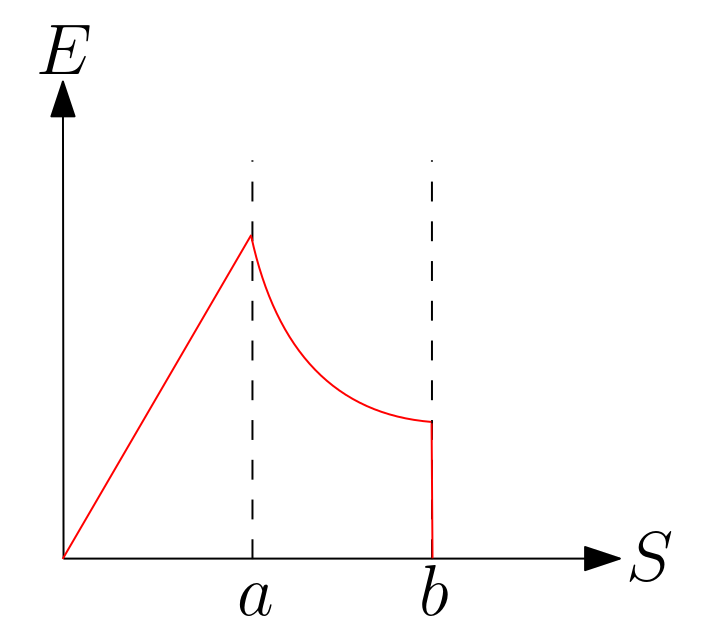
\includegraphics[width=0.5\linewidth]{PHYS350_Ass2_Figure.png}
					\captionsetup{margin=1cm, justification=raggedright}\caption{An approximate behaviour of $\vec{E}$ as a function of distance from the center.}
				\end{figure}
		\section*{Question 2.20}
			\subsection*{a) }
				\begin{equation}
					\left(\pdv{E_{z}}{y} - \pdv{E_{y}}{z}\right)\hat{x} - \left(\pdv{E_{z}}{x} - \pdv{E_{x}}{z}\right)\hat{y} + 	\left(\pdv{E_{y}}{x} - \pdv{E_{x}}{y}\right)\hat{z}
				\end{equation}
				Plugging the values in Equation $1$ yields 
				\begin{align*}
					\nabla \cross \vec{E} &= (0-ky)\hat{x} -(3kz -0) \hat{y} + (3kz-0 )\hat{z} \\
					&=-ky \hat{x} -kz \hat{y} +(k2y - kx)\hat{z} \neq \vec{0}
				\end{align*}
				We check for the second vector field using Equation $(1)$
				\begin{align*}
					\nabla \cross \vec{E} &= (2kz - 2kz) \hat{x} - (0+0)\hat{y} +(2ky - 2ky)\hat{z} = \vec{0}.
				\end{align*}
				We look for the potential using the line integral. Let $\vec{r} = (x,y,z)$, then by definition of the line integral 
				\begin{align*}
					V = -\int_{0}^{r} \vec{E} \cdot d\vec{l} &= -\int_{0}^{r} \vec{E}\cdot (dx\hat{x} +dy \hat{y} + dz\hat{z}) \\ 
					&= -\int_{0}^{r} (ky^{2}dx + (k2xy + kz^{2})dy + 2kyzdz)
				\end{align*}
				Let us integrate each component respectively with respect to their spatial components
				\begin{align*}
					&(x \neq 0) \quad V_{x} = - \int_{0}^{x} ky^{2}dx = 0 \\
					&(x \neq 0 \ , y \neq 0)  \quad V_{y} =-\int_{0}^{y} (k2xy+kz^{2})dy = -kxy^{2} \\
					&(x \neq 0 \ , y \neq 0 \ , z \neq 0) \quad V_{z} =- \int_{0}^{z} (2kyz)dz = -kyz^{2} 
				\end{align*}
				Finally, 
				$$ V = V_{x} + V_{y} + V_{z} = -kxy^{2} - kyz^{2} = -k(xy^{2} +yz^{2}).$$
				We verify that this is the right potential ,
				\begin{align*}
					\vec{E} = -\nabla V &= k \nabla (xy^{2} + yz^{2}) \\
					&= k(y^{2} \hat{x} + (2xy+z^{2})\hat{y} +2yz\hat{z}) \quad \checkmark.
				\end{align*}
		\section*{Question 2.34}
			\subsection*{a) }
				The potential inside the sphere is
				\begin{align*}
					V(r<R) &= - \int_{\infty}^{R} E_{\text{out}} dr - \int_{R}^{r} E_{\text{in}}dr \\
					&=-\int_{\infty}^{R} \frac{kQ}{R^{2}} dr - \int_{R}^{r} \frac{kgr}{R^{3}} dr \\
					&= \frac{kq}{R} - \frac{kq}{R^{3}} \Biggl[\frac{r^{2}}{2}\Big|_{R}^{r}\Biggr] \\
					&= \frac{kq}{R}(1-\frac{r^{2}}{2R^{2}} +\frac12) \\
					&= \frac{kq}{2R} \left(3- \frac{r^{2}}{R^{2}}\right).
 				\end{align*}
 				Next we compute using the Equation $2.43$.
 				\begin{align*}
 					\intertext{Since $V\rho = Q \implies \rho =\frac{3Q}{4 \pi R^{3}}$.}
 					W &= \frac12 \int \rho V \ d\tau \\
 					&= \frac12 \left(\frac{3Q}{4\pi R^{3}}\right)\frac{kQ}{2R} \int \left(3 - \frac{r^{2}}{R^{2}}\right) \ dr \\
 					\intertext{In spherical coordinates, the Jacobian is $r^{2}\sin\theta$.}
 					&=\frac12 \left(\frac{3Q}{4\pi R^{3}}\right)\frac{kQ}{2R} \int_{0}^{R}\int_{0}^{\pi} \int_{0}^{2\pi} \left(3 - \frac{r^{2}}{R^{2}}\right) r^{2} \sin \theta d\theta d\phi dr \\
 					&= \frac{4\pi}{2} \left(\frac{3Q}{4\pi R^{3}}\right)\frac{kQ}{2R} \int_{0}^{R} \left(3r^{2} - \frac{r^{4}}{R^{2}}\right) dr \\
 					&= \frac{36Q^{2} 4R^{5}}{4(16)R^{6}5} \\
 					&= \frac{3Q^{2}k}{5R}.
 				\end{align*}
 				\subsection*{b) }
 					First we find the inside and outisde electric fields. 
 					$$ E_{\text{in}} \to E(4\pi r^{2}) = \frac{Q}{\ep_{0}} \frac{r^{3}}{R^{3}} \implies E_{\text{in}} = \frac{Qr}{4\pi R^{3}\ep_{0}} \hat{r}.$$
 					Similarly, 
 					$$ E_{\text{out}} \to E(4\pi r^{2}) = \frac{Q}{\epsilon_{0}} \implies E_{\text{out}} = \frac{Q}{4\pi r^{2}\ep_{0}}\hat{r}.$$
 					Then we proceed with equation $2.45$.
 					\begin{align*}
 						W &= \frac{\ep_{0}}{2} \int (E_{\text{in}})^{2} \ d\tau + \frac{\ep_{0}}{2} \int (E_{\text{out}})^{2} \ d\tau \\
 						\intertext{Again we solve in polar coordinates.}
 						&= \frac{4\pi \ep_{0}}{2} \int_{0}^{R} \frac{r^{4}Q^{2}}{4^{2}\pi^{2}R^{6}\ep_{0}^{2}} \ dr + \frac{4\pi \ep_{0}}{2} \int_{0}^{R} \frac{Q^{2}}{4^{2}\pi^{2}r^{2}\ep_{0}^{2}} \ dr \\
 						&= \frac{4\pi \ep_{0}}{2} \Bigg[\frac{r^{5}Q^{2}}{5(4^{2}\pi^{2}R^{6}\ep_{0}^{2})}\Big|_{0}^{R}\Bigg] + \frac{4\pi \ep_{0}}{2} \Bigg[\frac{-Q^{2}}{4^{2}\pi^{2}r\ep_{0}^{2}}\Big|_{R}^{\infty}\Bigg] \\
 						&=\frac{\ep_{0}4\pi}{2} \left(\frac{6Q^{2}}{5R(4^{2}) \pi^{2}\ep_{0}^{2}}\right) \\
 						&= \frac{3Q^{2}k}{5R}.
 					\end{align*}
 				\section*{Question 2.35}
 					We know that
 					$$ Q = \rho V \implies dQ = \rho dV = \rho A dr = \rho (4\pi r^{2} dr).$$
 					The volume charge density over a sphere is 
 					$$\rho = \frac{3q}{4\pi R^{3}} \implies dq =\frac{3q r^{2}}{R^{3}} \ dr. $$
					To move a unit  charge from reference point at the infinity, 
					$$ W = QV(\vec{r}) \implies dW = V_{\text{out}} dQ$$. 
					\begin{gather*}
						E_{\text{in}} \to E(4\pi r^{2}) = \frac{Q_{\text{enc}}}{\ep_{0}} \implies E_{\text{in}} = \frac{Q}{4\pi \ep_{0}r^{2}} \hat{r}. \\
						V_{\text{out}} = - \int_{\infty}^{r} \frac{Q}{4\pi \ep_{0} r^{2}} \ dr = \frac{kQ}{r}.
					\end{gather*}
					Finally , 
					\begin{align*}
						dW &= \frac{kQ_{\text{enc}}}{r} dQ \\
						dW &= \frac{3QkQ_{\text{enc}}r}{R^{3}} dr
						\intertext{Since the charge insite $Q_{\text{enc}}$ is the ratio of the two volumes it follows that $Q_{\text{enc}} = r^{3}Q/R^{3}$.}
						dW &= \frac{r^{4}}{R^{6}} 3Q^{3} k \ dr.
						\intertext{This is the infinitesimal work for a infinitesimal $dr$ radius. Now integrating, }
						W &= \int_{0}^{R} \frac{r^{4}}{R^{6}}  3Q^{2} k \ dr = \frac{3Q^{2}}{5R}.
					\end{align*}
				\section*{Question 2.46}
				We use the Poisson's equation $\nabla \cdot \vec{E} = \rho / \ep_{0}$. Then use the divergence in spherical coordinates relationship. 
				\begin{align*}
					\rho &= \frac{-k\ep_{0}}{r} \Bigg[\frac{1}r^{2} \pdv{E_{r} r^{2}}{r} + \frac{1}{r\sin\theta} \pdv{E_{\theta} \sin \theta}{\theta} + \frac{1}{r\sin\theta} \pdv{E_{\phi}\phi}{\phi} \Bigg] \\
					&=\Bigg[\frac{3k}{r^{2}} +\frac{\partial }{\partial \theta} \left(\frac{\sin \theta (2k \sin \theta \cos \theta \sin \phi)}{r}\right) -\frac{\sin\phi}{r^{2}}\Bigg] \\
						&=\Bigg[\frac{3k}{r^{2}} +\frac{2k}{r} \sin \phi \left(\frac{\partial }{\partial \teta} \left(\sin^{2} \theta\right)\cos \theta + \frac{\parital }{\partial \theta} \left(\cos \theta\ \sin^{2}\theta \right)\right) -\frac{\sin\phi}{r^{2}}\Bigg] \\
						&=\Bigg[\frac{3k}{r^{2}} +\frac{2k \sin \phi }{r^{2}} \left(2 \cos^{2} \theta - \sin^{2}\theta \right) -\frac{\sin\phi}{r^{2}}\Bigg] \\
						&=\frac{k\ep_{0}}{r^{2}} \left(3+ 2\sin\phi(2\cos^{2}\theta - \sin^{2} \theta) - \sin\phi\right)\\
						&=\frac{k\ep_{0}}{r^{2}} (3 + \sin \phi(4 \cos^{2}\theta - 2\sin^{2}\theta -1 )) \\
						&=\frac{3k\ep_{0}}{r^{2}} (1 + \sin\phi(2\cos^{2}\theta - 1)) \quad \checkmark. 
				\end{align*}
			\section*{Question 6}
				Let $r'$ be the radius of a Gaussian sphere, $r$ the radius for the inside cavity and $R$ the radius for the main sphere. 
				\subsection*{a) }
					For the first part of the question we ignore the inside cavity, 
					\begin{align*}
						E(4\pi r'^{2}) = \frac{Q_{\text{enc}}}{\ep_{0}} \implies E_{\text{in}} &= \frac{Qr'^{3}}{4\pi r'^{2} R^{3} \ep_{0}} \\
						&=\frac{Qr'}{4 \pi R^{3} \ep_{0}}
						\intertext{Since $\rho = \frac{3Q}{4\pi R^{3}}$, this results to}
						\vec{E_{\text{in}}} &= \frac{\rho r^{\prime}}{3\ep_{0}}\hat{r'}, 
					\end{align*}
					is the electric field inside the sphere but outside the cavity ,where $0 < r' < R$.
				\subsection*{b) }
					By the superposition principle the inside cavity has negative charge density.Setting the endpoint of $r'$ near the edge of $B_{r}$, it follows from vector addition that $r' + r = d$, from the superposition of the electric fields, 
					\begin{gather*}
						\vec{E} = \vec{E_{+}} + \vec{E_{-}} \\
						\therefore \vec{E} = \frac{\rho r'}{3 \ep_{0}} \hat{r'} + \frac{-\rho r}{3 \ep_{0}} \hat{r} = \frac{\rho d}{3 \ep_{0}}\hat{d} .
					\end{gather*}
			\section*{Question 7}
				\subsection*{a) }
					\begin{gather*}
						V = W/Q \implies V = 10^{4} \ \si{\volt}.
					\end{gather*}
				\subsection*{b) }
					V = $\frac{kQ}{R_{e}} = 10^{4} \implies Q = \frac{10^{4} \cross 6371 \cross 10^{3}}{8.987\cross 10^{9}} = 7.09 \ \si{\coulomb}$.
					For this quantity of charge ,
					\begin{gather*}
						7.09 \ \si{\coulomb} \implies 4.43 \cross 10^{19} \ \text{e}. \\
						\therefore (4.43 \cross 10^{19})m_{p} = 4.43 \cross 10^{19} \cross 1.67 \cross 10^{-27} = 7.38 \cross 10^{-8} \ \si{\kilogram}.
					\end{gather*}
				\subsection*{c) }
					$4$ atoms per $\si{\centi\meter\cubed}$ is equivalent to $4\cross 10^{6}$ atoms per $\si{\meter\cubed}$. The distance from earth to sun is $150 \cross 10^{9} \ \si{\meter}$. If it takes $3$ days for a particle to reach the earth then the speed is $50 \cross 10^{9} \ \si{\meter\per\day}$. Converting in meter per second we have $v \approx 6 \cross 10^{5} \ \si{\meter\per\second}$.
					
					\noindent Whenever one meter cube of space hit one meter squared of the earth with one second, $4\cross 10^{6}$ particles hit that one meter square. Therefore for every second ,
					$$ (6\cross 10^{5})(4\cross 10^{6})(1.672\cross 10^{-27}) = 4.01\cross 10^{-15} \ \si{\kilogram\per\meter\squared\per\second}.$$
					We take half the surface of the earth and multiply by the rate above we get that the rate at which mass is deposited on the Earth is 
					$$ (4.01\cross 10^{-15})(2\pi R_{e}^{2}) = 1.02 \ \si{\kilogram\per\second}.$$
					
					\noindent Finally, the time $T$ for $7.38 \cross 10^{-8} \ \si{\kilogram}$ is 
					$$ T = \frac{7.38 \cross 10^{-8} \ \si{\kilogram}}{1.02 \ \si{\kilogram\per\second}} \approx 7.2 \cross 10^{-8} \ \si{\second}.$$
					
				\subsection*{d) }
					The reason why we nevertheless see the auroras is because the protons aren't roaming freely in space, they come in atoms and hence with other electrons. These atoms are mostly electrically neutral (not charged) and so they don't get repelled. 
			\section*{Bonus }
			\begin{figure}[H]
				\centering
				\includegraphics[width=0.8\linewidth]{PHYS350_bonus.png}
			\end{figure}
				\begin{figure}[H]
					\centering
					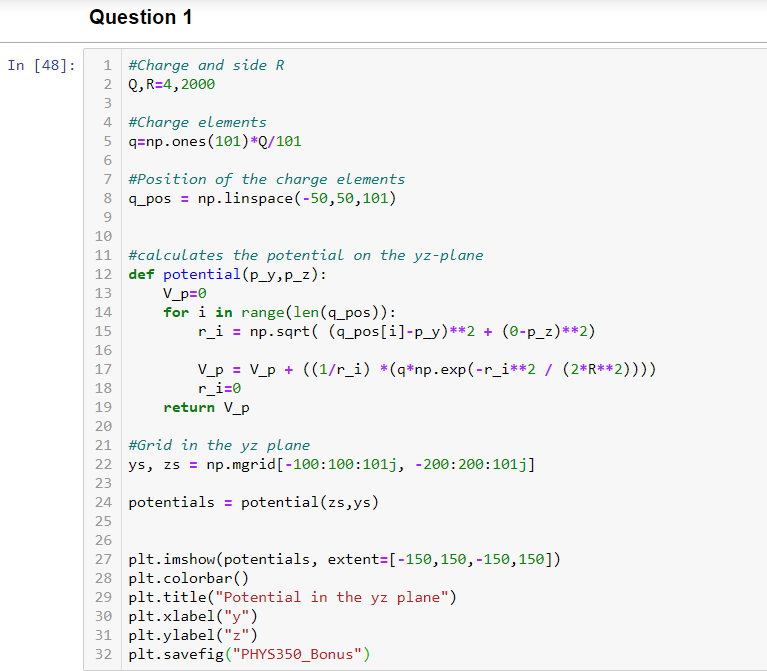
\includegraphics[width=1.0\linewidth,height=1.0\linewidth]{PHYS350_1.png}
				\end{figure}
	\end{document}